\documentclass[tikz,border=10pt]{standalone}
\usepackage{tikz}
\usetikzlibrary{calc,angles,intersections}

\begin{document}
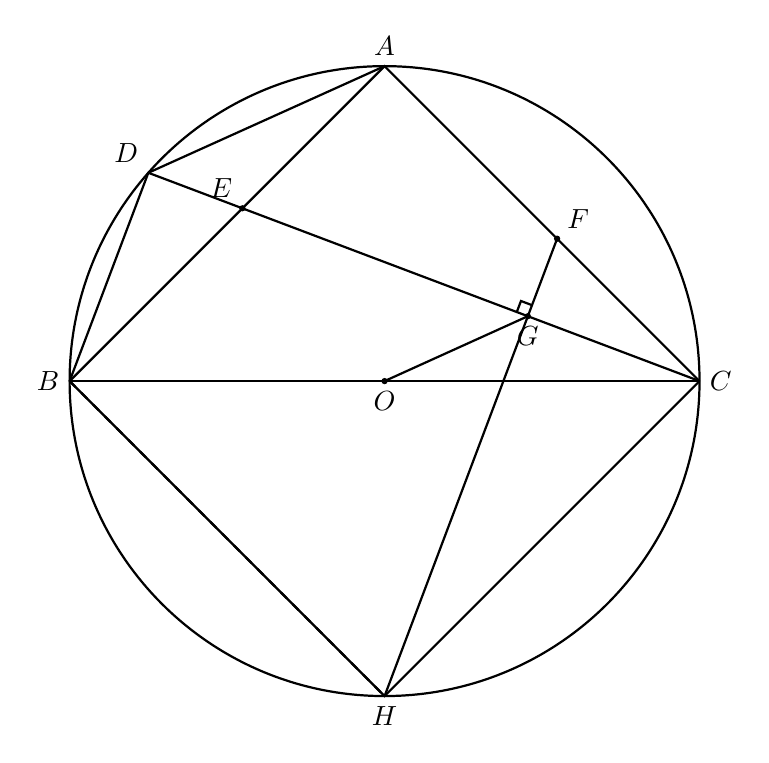
\begin{tikzpicture}[scale=2, line width=0.8pt]
  % 定义基础点：BC为直径，圆心O
  \coordinate (B) at (-2,0);
  \coordinate (C) at (2,0);
  \coordinate (O) at (0,0);   % 圆心
  
  % 圆上各点坐标
  \coordinate (A) at (0,2);    % 上顶点
  \coordinate (D) at (-1.5, {sqrt(4 - 1.5*1.5)}); % 左上圆上点
  \coordinate (H) at (0,-2);  % 下顶点
  
  % 绘制外接圆（以O为圆心，半径为2）
  \draw (O) circle (2);
  
  % 绘制实线
  \draw (B) -- (C);           % 直径BC
  \draw (B) -- (A) -- (C);    % 三角形ABC
  \draw (B) -- (D) -- (A);    % 线段BD、DA
  \draw (D) -- (C);           % 线段DC
  \draw (C) -- (H) -- (B);    % 线段CH、HB
  
  % 定义交点E（AB与CD的交点）
  \coordinate (E) at (intersection of A--B and C--D);
  
  % 在CA上截取CF = AE
  % 使用 let 语法计算比例
  \path let \p1 = ($(E)-(A)$),      % 向量 AE
            \p2 = ($(A)-(C)$),      % 向量 CA（从C到A）
            \n1 = {veclen(\x1,\y1)}, % AE 的长度
            \n2 = {veclen(\x2,\y2)}, % CA 的长度
            \n3 = {\n1/\n2}         % 比例 = AE/CA
        in ($(C) + \n3*($(A)-(C)$)$) coordinate (F);
  
  % 过F作GF垂直CD于点G
  \coordinate (G) at ($(C)!(F)!(D)$);
  
  % 绘制线段FG（垂直于CD）
  \draw (F) -- (G) -- (H);
  \draw (O) -- (G);
  
  % 绘制虚线辅助线
  \draw[dashed] (B) -- (H);   % 辅助线BH
  
  % 绘制直角符号（FG⊥CD）
  \pic [draw, angle radius=0.15cm] {right angle = F--G--D};
  
  % 标注所有顶点
  \node[above] at (A) {$A$};
  \node[left] at (B) {$B$};
  \node[right] at (C) {$C$};
  \node[below] at (O) {$O$};
  \node[above left] at (D) {$D$};
  \node[above right] at (F) {$F$};
  \node[above left] at (E) {$E$};
  \node[below] at (H) {$H$};
  \node[below] at (G) {$G$};
  
  % 绘制点标记
  \fill (O) circle (0.02);
  \fill (E) circle (0.02);
  \fill (F) circle (0.02);
  \fill (G) circle (0.02);
\end{tikzpicture}
\end{document}